\documentclass[10pt, a4paper]{article}
\usepackage[utf8x]{inputenc}            % Acentos, ñ, etc.
\usepackage{graphicx}                   % Gráficos
\usepackage[spanish]{babel}             % Macros en español
\usepackage{caratula}                   % Carátula
\usepackage{float}
\usepackage[paper=a4paper, left=2cm, right=2cm, bottom=2cm, top=3.5cm]{geometry}
\begin{document}

%Caratula
\titulo{Trabajo Práctico 1 - Reentrega}
\subtitulo{Detección de Spam}
\fecha{\today}
\materia{Aprendizaje Automático}
\integrante{Fernández, Gonzalo}{836/10}{gpfernandezflorio@gmail.com}
\integrante{Damian, Aleman}{377/10}{damianealeman@gmail.com}
\integrante{Matías, Pizzagalli}{257/12}{matipizza@gmail.com}

%Titulo e indice
\maketitle
\tableofcontents
\newpage

\section{Introducción}

Este trabajo práctico consiste en analizar distintas estrategias para implementar un algoritmo de reconocimiento de spam utilizando técnicas de clasificación de aprendizaje supervisado. El objetivo es obtener un programa que lea el contenido de un correo electrónico y logre clasificarlo correctamente como \texttt{ham} o \texttt{spam}. Para lograrlo, debemos entrenar a los algoritmos con una base de correos etiquetados, provista por la cátedra de la materia.

\section{Metodología}

Para entrenar satisfactoriamente un algoritmo de aprendizaje supervisado, lo primero que se debe hacer es determinar los atributos que el algoritmo debe tener en cuenta para clasificar instancias. En el problema de detección de spam, estos atributos podrían ser la cantidad de apariciones de determinadas palabras. Si bien podríamos pensar cuáles podrían ser esas palabras, se nos ocurrió hacer un programa que las identifique. En otras palabras, hicimos un script que \textit{elige} los atributos que vamos a seleccionar. En la primera entrega cometimos el error de ejecutar este script sobre toda la base de entrada, antes de retirar una fracción de ella para validación. Esto provocó que la base de validación no cumpliera su objetivo de contener datos frescos.
Para la reentrega, invertimos el orden de esas acciones, ignorando completamente cualquier resultado anterior. Además, dividimos el script principal en varios subscripts, cada uno con una funcionalidad específica correspondiente a un paso del desarrollo del trabajo. En el archivo \texttt{README.md} figuran las instrucciones con el modo de uso y la descripción de cada script.

\subsection{Base de validación}

El primer paso del desarrollo de este trabajo práctico es la extracción del conjunto de datos para validación. El script \texttt{cortaBase.py} carga los archivos de la base \texttt{ham\_dev.json} y \texttt{spam\_dev.json}, genera un único dataframe etiquetado y extrae un $20\%$ del mismo como base de validación. Esta se almacena en el archovo \texttt{test.npy}, mientras que el resto de la base, la base de desarrollo se almacena en el archivo \texttt{train.npy}. Ahora sí podemos elegir los atributos para el entrenamiento, a partir de analizar los correos en la base de desarrollo.

\subsection{Selección de atributos}

El script \texttt{wordCounter.py} lee la base de desarrollo \texttt{train.npy} y cuenta la cantidad de apariciones de cada palabra en cada clase. Al final decidimos quedarnos con los atributos correspondientes a la cantidad de apariciones de 200 palabras:

\begin{itemize}
\item De las palabras que sólo aparecen en la clase spam, las 100 con mayor cantidad de apariciones.
\item De las palabras que aparecen en ambas clases, las 100 con mayor proporción de apariciones en spam sobre apariciones en ham.
\end{itemize}

Este script genera el archivo \texttt{attributes.py} que contiene las variables y funciones necesarias para extraer los atributos de cada instancia. También utilizamos el atributo longitud.

Por otro lado, el script \texttt{cargaAtributos.py} toma la base de desarrollo \texttt{train.npy} y la convierte en una matriz de instancias por atributos utilizando los atributos designados en \texttt{attributes.py}. Almacena esta matriz en el archivo \texttt{trainX.npy} y el vector de etiquetas en el archivo \texttt{trainy.npy}. Luego hace lo mismo con la base de validación, almacenando el resultado en los archivos \texttt{testX.npy} y \texttt{testy.npy}. De esta forma, la dejamos formateada para cuando la necesitemos al final de la experimentación.

\subsection{Reducción de dimensionalidad}

El siguiente paso consiste en obtener bases de desarrollo y validación con menor cantidad de atributos, pero con la misma cantidad de información (o reduciendo todo lo posible la pérdida de información). Para ello se utilizaron dos técnicas de reducción de dimensionalidad. El script \texttt{reducirDimensiones.py} toma las matrices de atributos \texttt{trainX.npy} y \texttt{testX.npy} y las reduce aplicando alguna de estas dos técnicas. Toma como parámetros el método a utilizar (PCA o ICA) y la cantidad de componentes (10 por defecto). Almacena las matrices resultantes en archivos llamados \texttt{M.n.npy} y \texttt{M.n-test.npy} siendo \texttt{M} el método y \texttt{n} la cantidad de componentes.

Mediante el uso de este script se generaron 22 bases reducidas (11 con PCA y 11 con ICA). Las cantidades de componentes utilizadas fueron 1, 2, 3, 4, 5, 10, 20, 40, 60, 80 y 100.

\subsection{Modelos} \label{modelos}

Antes de entrenar los modelos sobre las bases, debimos determinar los mejores hiperparámetros para cada modelo. Eso lo hace el script \texttt{gridSearch.py} que toma como parámetros un método y una base y escribe en un archivo los mejores parámetros obtenidos haciendo grid search sobre ese modelo. El nombre del archivo consiste en el nombre del método seguido de un punto, seguido del nombre de la base.
A continuación se detallan los algoritmos utilizados junto con los valores explorados para cada uno de sus hiperparámetros.

\begin{itemize}
\item Árbol de Decisión (implementado con la clase \textbf{DecisionTreeClassifier}) \\
  Hiperparámetros:
  \begin{itemize}
    \item \textbf{max\_depth}: 1, 5, 10, 15, 20, None
    \item \textbf{max\_features}: 1, 50, 100, 150, None
    \item \textbf{min\_samples\_split}: 1, 2, 3, 4, 5
    \item \textbf{criterion}: entropy, gini
  \end{itemize}
\item Random Forest (implementado con la clase \textbf{RandomForestClassifier}) \\
  Hiperparámetros:
  \begin{itemize}
    \item \textbf{max\_depth}: 1, 5, 10, 15, 20, None
    \item \textbf{max\_features}: 1, 50, 100, 150, None
    \item \textbf{min\_samples\_split}: 1, 2, 3, 4, 5
    \item \textbf{criterion}: entropy, gini
    \item \textbf{n\_estimators}: 10, 50, 100, 150
  \end{itemize}
\item Naive Bayes (implementado con la clase \textbf{GaussianNB})
\item Vecinos más Cercanos (implementado con la clase \textbf{KNeighborsClassifier}) \\
  Hiperparámetros:
  \begin{itemize}
    \item \textbf{n\_neighbors}: 1, 2, 3, 4, 5
    \item \textbf{weights}: uniform, distance
  \end{itemize}
\item Support Vector Machines (implementado con la clase \textbf{SVC}) \\
  Hiperparámetros:
  \begin{itemize}
    \item \textbf{kernel}: linear, poly, rbf, sigmoid
    \item \textbf{max\_iter}: 10, 50, 100, 500, 1000
  \end{itemize}
\end{itemize}

Una vez definidos los mejores parámetros de cada método, pasamos a la parte de evaluar los modelos según las distintas métricas vistas en clase. El script \texttt{validar.py} ejecuta cross validation sobre un modelo y una base para luego escribir en el archivo \texttt{cv.txt} el tiempo que le demoró entrenar al modelo y las medias y varianzas de cada una de las métricas. Los valores de las métricas se calcularon utilizando \textit{spam} como la etiqueta positiva. La información contenida en este archivo será utilizada luego para generar los gráficos de la sección \textbf{Resultados}. El script toma como parámetros el método, la base y la cantidad de folds (10 por defecto).

A partir de los resultados obtenidos, determinaremos sobre qué base se comporta mejor cada algoritmo. Entonces pasaremos a guardar los modelos entrenados. El script \texttt{entrenar.py} toma un método y una base y almacena en un archivo el modelo entrenado en esa base. Estos modelos entrenados pueden utilizarse para clasificar nuevas instancias con el script \texttt{predecir.py} que toma como parámetro un archivo \texttt{.pickle} y una base y devuelve el vector de etiquetas para cada instancia de la base. Además, si se le pasa también un vector de etiquetas como parámetro, escribe en un archivo los valores de las métricas. Este script lo usaremos al final de la experimentación para clasificar las instancias en la base de validación.

\subsection{Gráficos}

Finalmente, tenemos el script \texttt{ploter.py} que lee el archivo \texttt{cv.txt} generado en la fase de cross validation y genera los archivos \texttt{.dat} que utilizará gnuplot para graficar toda esta información. En la carpeta \texttt{data} se encuentran todos los archivos de datos correspondientes y los archivos de gnuplot necesarios para volver a generar los gráficos.

\section{Resultados y Análisis}

\subsection{Grid Search}
En la siguiente tabla se muestran los mejores hiperparámetros obtenidos con cada método sobre cada base\footnote{Se omite la columna \texttt{weights} del método \textbf{KNN} ya que en todos los casos el resultado obtenido para dicho parámetro fue \texttt{distance}.}.Los resultados que aquí se muestran fueron obtenidos ejecutando el script \texttt{gridSearch.py}, descripto en la sección \ref{modelos}.
\\\\

\begin{scriptsize}
\begin{tabular}{|r|l||c|c|c|c||c|c|c|c|c||c||c|c|}
\hline
\multicolumn{2}{|c||}{ } & \multicolumn{4}{|c||}{Árbol de Decisión} & \multicolumn{5}{|c||}{Random Forest} & KNN & \multicolumn{2}{|c|}{SVM}\\
\hline
\multicolumn{2}{|c||}{ } & \rotatebox{270}{max\_depth} & \rotatebox{270}{max\_features} & \rotatebox{270}{min\_samples\_split} & \rotatebox{270}{criterion} & \rotatebox{270}{max\_depth} & \rotatebox{270}{max\_features} & \rotatebox{270}{min\_samples\_split} & \rotatebox{270}{criterion} & \rotatebox{270}{n\_estimators} & \rotatebox{270}{n\_neighbors} & \rotatebox{270}{kernel} & \rotatebox{270}{max\_iter} \\
\hline
\multicolumn{2}{|c||}{trainX} & None & 100 & 5 & entropy & None & 1 & 5 & entropy & 150 & 2 & rbf & 1000\\
\hline
PCA & 1 & 10 & None & 1 & gini & 10 & None & 1 & gini & 150 & 5 & poly & 1000 \\
\hline
PCA & 2 & None & None & 2 & gini & 20 & 1 & 2 & gini & 150 & 2 & rbf & 1000 \\
\hline
PCA & 3 & None & None & 1 & entropy & None & None & 1 & entropy & 100 & 2 & sigmoid & 10 \\
\hline
PCA & 4 & 20 & None & 1 & gini & None & 1 & 1 & gini & 150 & 2 & sigmoid & 10 \\
\hline
PCA & 5 & None & None & 1 & entropy & None & None & 1 & entropy & 150 & 2 & poly & 1000 \\
\hline
PCA & 10 & 20 & None & 1 & entropy & 20 & 1 & 1 & entropy & 150 & 2 & rbf & 1000 \\
\hline
PCA & 20 & 20 & None & 2 & gini & 20 & 1 & 2 & gini & 150 & 2 & rbf & 1000 \\
\hline
PCA & 40 & 20 & None & 1 & entropy & 20 & None & 1 & entropy & 150 & 2 & linear & 500 \\
\hline
PCA & 60 & 20 & 50 & 2 & entropy & 20 & 50 & 2 & entropy & 150 & 2 & rbf & 1000 \\
\hline
PCA & 80 & 20 & 50 & 4 & gini & 20 & 50 & 4 & gini & 150 & 2 & rbf & 1000 \\
\hline
PCA & 100 & 15 & None & 1 & gini & 20 & 50 & 1 & gini & 150 & 2 & rbf & 500 \\
\hline
ICA & 1 & 5 & None & 1 & entropy & 5 & None & 1 & entropy & 10 & 3 & linear & 10 \\
\hline
ICA & 2 & None & None & 2 & entropy & None & None & 2 & entropy & 50 & 5 & linear & 10 \\
\hline
ICA & 3 & None & None & 2 & gini & 20 & None & 2 & gini & 150 & 5 & linear & 10 \\
\hline
ICA & 4 & None & None & 4 & gini & None & None & 4 & gini & 100 & 4 & linear & 10 \\
\hline
ICA & 5 & None & None & 3 & entropy & None & None & 3 & entropy & 100 & 4 & linear & 500 \\
\hline
ICA & 10 & 20 & None & 3 & entropy & 20 & None & 3 & entropy & 100 & 4 & linear & 1000 \\
\hline
ICA & 20 & 20 & None & 3 & entropy & None & 1 & 3 & entropy & 150 & 4 & linear & 100 \\
\hline
ICA & 40 & 20 & None & 3 & entropy & 20 & None & 3 & entropy & 150 & 4 & linear & 10 \\
\hline
ICA & 60 & 20 & 50 & 1 & entropy & 20 & 50 & 1 & entropy & 150 & 5 & linear & 10 \\
\hline
ICA & 80 & 20 & None & 3 & gini & 20 & 50 & 3 & gini & 150 & 4 & linear & 10 \\
\hline
ICA & 100 & 20 & None & 5 & gini & 20 & 50 & 5 & gini & 150 & 4 & linear & 10 \\
\hline
\end{tabular}
\end{scriptsize}

Notamos que el kernel de SVM elegido por GridSearch para las bases generadas con ICA es lineal en todos los casos.
Por otro lado, nos llamó la atención que en la base con todos los atributos el método de random forest según GridSearch tiene como valor óptimo del atribiuto max\_features es 1, mientras que con el método de Decision Tree, a este atributo casi siempre se le asignaba el valor None (ningún máximo).

\subsection{Cross Validation}

Las siguientes referencias valen para todos los gráficos de esta sección. Los resultados que aquí se muestran fueron obtenidos ejecutando el script \texttt{validar.py}, descripto en la sección \ref{modelos}.

\begin{figure}[H]
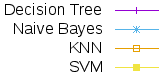
\includegraphics[scale=0.6]{../src/data/refs.png}
\end{figure}

\subsubsection{Tiempos de ejecución}

Una característica importante de los modelos es el tiempo necesario para entrenar. Si bien no es crucial que se entrenen en poco tiempo, tampoco queremos esperarlo por siempre. Una de las cosas que mide el script \texttt{validar.py} al hacer Cross Validation, es la cantidad de segundos que dura la ejecución del método \texttt{fit}.

En los siguientes gráficos se muestra la cantidad de tiempo en segundos que demoró cada método en entrenar sobre cada base. Cada punto corresponde al promedio de las 10 iteraciones de Cross Validation. También se grafica la varianza, aunque en la mayoría de los casos es casi inperceptible.

\begin{figure}[H]
\centering
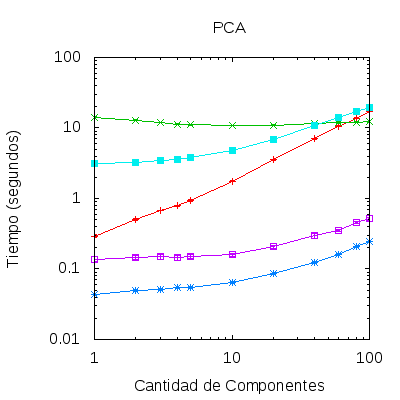
\includegraphics[scale=0.6]{../src/data/tmpca.png}
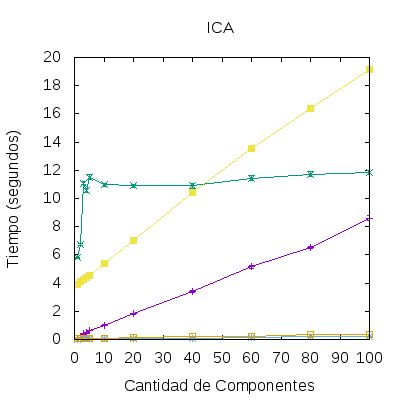
\includegraphics[scale=0.6]{../src/data/tmica.png}
\end{figure}

Tanto en las bases generadas con PCA como en las generadas por ICA, el tiempo de entrenamiento es creciente en función de la cantidad de componentes para todos los métodos, excepto Random Forest, el cual parece durar menos a mayor cantidad de componentes.

Ahora veamos cómo se comportan estos métodos sobre la base completa, sin reducir la dimensionalidad.

\begin{figure}[H]
\centering
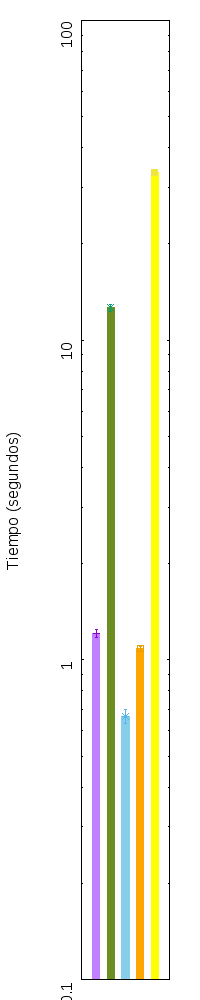
\includegraphics[scale=0.6,angle=-90]{../src/data/tm.png}
\end{figure}

\subsubsection{Performance}

Sobre cada fold de Cross Validation, el script \texttt{validar.py} calcula 5 métricas de performance vistas en clase. Estas son \textit{Precision}, \textit{Accuracy}, \textit{Recall}, \textit{F1} y \textit{ROC Area Under Curve}. Si bien generamos los gráficos para cada una de estas métricas, los gráficos de \textit{Accuracy} resultaron ser casi idénticos a los de \textit{ROC Area Under Curve}, con lo cual nos quedamos sólo con el primero. El resto de los gráficos pueden encontrarse en la carpeta \texttt{src/data}

En los siguientes gráficos se muestran los valores de \textit{Precision}, \textit{F1} y \textit{ROC Area Under Curve} para cada modelo comparando entre las bases generadas por \textit{PCA} y por \textit{ICA}. Una vez más, cada punto corresponde al promedio y la varianza de las 10 iteraciones del Cross Validation sobre una determinada base. El eje x (cantidad de componentes) está en escala logarítmica.

\begin{figure}[H]
  \begin{minipage}{1\textwidth}
  \center PCA\\
	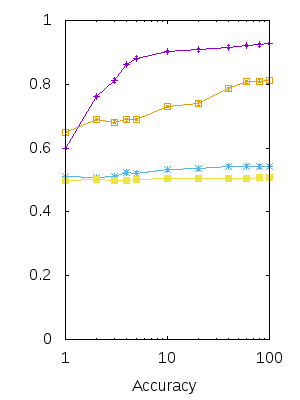
\includegraphics[scale=0.5]{../src/data/acpca.png}
	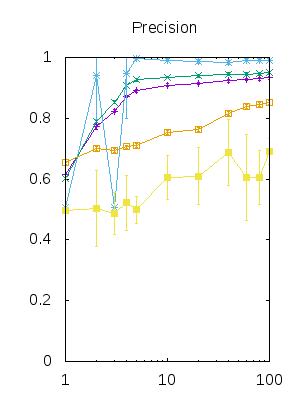
\includegraphics[scale=0.5]{../src/data/prpca.png}
	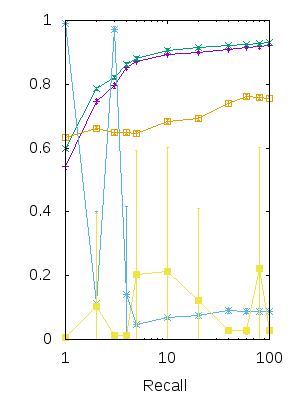
\includegraphics[scale=0.5]{../src/data/repca.png}
	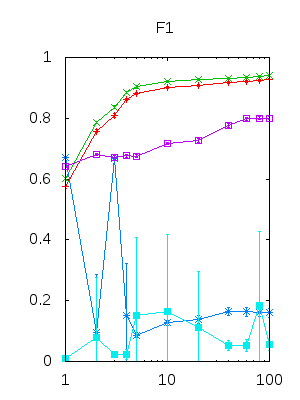
\includegraphics[scale=0.5]{../src/data/f1pca.png}
  \center ICA\\
	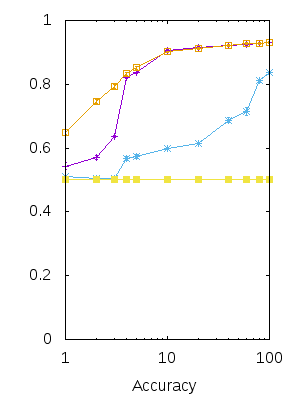
\includegraphics[scale=0.5]{../src/data/acica.png}
	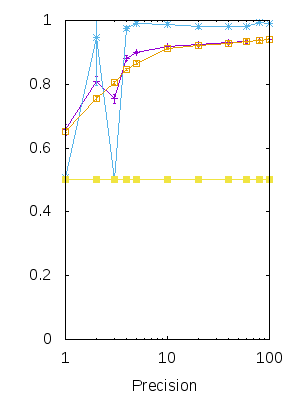
\includegraphics[scale=0.5]{../src/data/prica.png}
	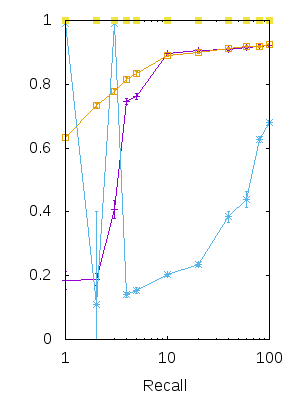
\includegraphics[scale=0.5]{../src/data/reica.png}
	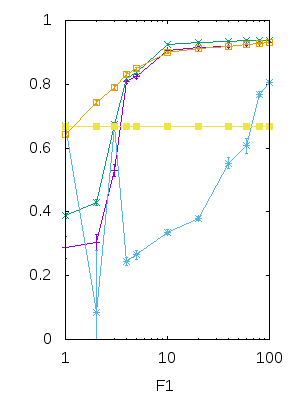
\includegraphics[scale=0.5]{../src/data/f1ica.png}
  \end{minipage}
\end{figure}

En general, todos los métodos tienden a mejorar a médida que se incrementa la cantidad de componentes, aunque este incremento se torna despreciable a partir de la décima componente. En los gráficos de accuracy se ve claramente esta tendencia.

El método de Naive Bayes es la excepeción.
En el caso de las bases generadas con PCA la métrica de accuracy es bastante baja sin importar la cantidad de componentes.
Sin embargo, en el caso generado con ICA sí se nota el incremento en accuracy incluso después de la décima componente. Esto tiene sentido, ya que Naive Bayes asume que los atributos son independientes, y no necesariamente lo son. Como el método ICA genera componentes independientes, Naive Bayes tiene mejores resultados a diferencia de PCA. Este mismo patrón puede verse en los gráficos de recall y f1 de ICA.

Por otro lado, notamos que el método de SVM es altamente variable en la mayoría de las métricas sobre PCA. Es decir, que cada en cada fold se obtuvieron resultados muy dispares. Es curiosos considerando que en el resto de los casos la varianza es imperceptible. Otra particularidad de este método es

Ahora veamos cómo se comportan estos métodos sobre la base completa, sin reducir la dimensionalidad.

\begin{figure}[H]
  \begin{minipage}{1\textwidth}
	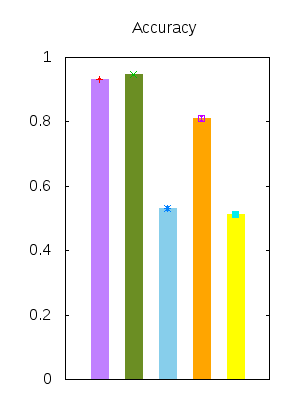
\includegraphics[scale=0.5]{../src/data/ac.png}
	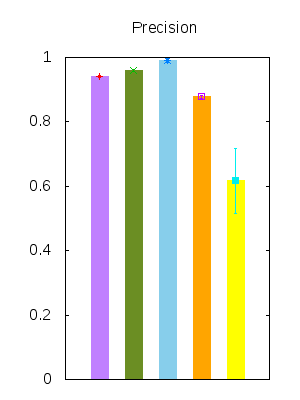
\includegraphics[scale=0.5]{../src/data/pr.png}
	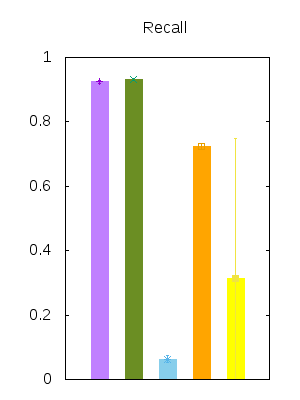
\includegraphics[scale=0.5]{../src/data/re.png}
	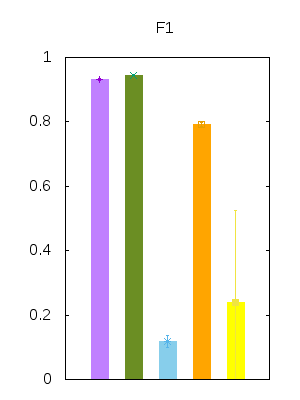
\includegraphics[scale=0.5]{../src/data/f1.png}
  \end{minipage}
\end{figure}

\subsection{Validación}

A partir de los resultados obtenidos en la sección anterior elegimos una base para cada método y lo entrenamos sobre esa base con el script \texttt{entrenar.py}. Decidimos basarnos principalmente en la métrica F1 para decidir qué base utilizar para cada método. Observando de cerca los gráficos (y los .dat que los generaron)determinamos...

Luego utilizamos el script \texttt{predecir.py} para ejecutar, sobre la base de validación, cada clasificador entrenado.

\section{Conclusiones}

Después de notar que SVM tiene un recall casi perfecto en las bases de ICA para cualquier cantidad de componentes,
mientras que sus valores de Accuracy y Precision apenas superaban 0.5, concluímos que es importante tener en cuenta todas las métricas a 
la hora de evaluar que tan bueno es un clasificador ya que restringirnos a una sola podría llevarnos a sobrestimar un clasificador.




\end{document}
